\newsavebox\exnotebox
\begin{lrbox}{\exnotebox}
  \begin{minipage}{6.5cm}
    %% dont re-indent this file
\begin{lstlisting}[style=scalaioScala]
val I:Rte = Atomic(classOf[Int])
val F:Rte = Atomic(classOf[Float])
val D:Rte = Atomic(classOf[Double])

val re:Rte = (I ++ (D | F).+).*
\end{lstlisting}

  \end{minipage}
\end{lrbox}


\begin{frame}{RTEs}{What are Regular Type Expressions?}
  \begin{columns}
    \begin{column}{0.55\textwidth}
  \begin{itemize}
  \item An RTE is an \Emph{expression} designating a set  of finite sequences
  \item Describes regular \emph{type patterns} sequence content.
  \item RE-matching is a \Emph{set membership} check.
  \item Mathematical notation: $(Int \cdot (Double \cup Float)^+)^*$
  \item Scala notation\\
    \usebox\exnotebox
  \end{itemize}
    \end{column}%
    \begin{column}{0.45\textwidth}
      \scalebox{0.7}{% Modeled after the following
% A simple Tree
% Author: Stefan Kottwitz
% https://www.packtpub.com/hardware-and-creative/latex-cookbook
\documentclass[border=10pt]{standalone}
\usepackage{tikz}
\begin{document}
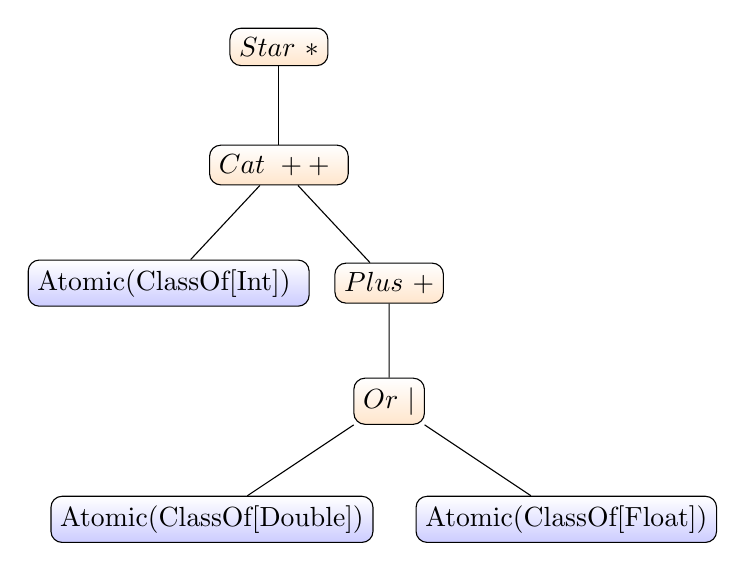
\begin{tikzpicture}[sibling distance=10em,
  every node/.style = {shape=rectangle, rounded corners,
    draw, align=center,
    top color=white, bottom color=orange!20}]]
    \tikzstyle{level 2}=[sibling distance=28mm]
    \tikzstyle{level 4}=[sibling distance=45mm]
  \node {$Star~*$}
  child { node { $Cat~++$ } 
    child { node [bottom color=blue!20] {\text{Atomic(ClassOf[Int])} }}
    child { node {$Plus~+$} 
      child { node {$Or~|$}
        child { node [bottom color=blue!20] {\text{Atomic(ClassOf[Double])}} }
        child { node [bottom color=blue!20] {\text{Atomic(ClassOf[Float])}} } } } } ;
\end{tikzpicture}
\end{document}
}
    \end{column}%
  \end{columns}%
\end{frame}


\newsavebox\exampleAbox
\begin{lrbox}{\exampleAbox}
  \begin{minipage}{12cm}
    %% dont re-indent this file
\begin{lstlisting}[style=scalaioScala]
val data = Seq("C", 100, 200, 300,
               "M", 10.0, 20.0,
               "M",
               "C", 1, 2, 3,
               "C", -1, -3, -7, -8)
\end{lstlisting}

  \end{minipage}
\end{lrbox}



\begin{frame}{Example 2}{An RTE to match}
  \usebox\exampleAbox

  \begin{itemize}
  \item Keyword strings \code{"C"} (counts) and \code{"M"} (measurements)
  \item \code{"C"} followed by zero or more \code{Int} values
  \item \code{"M"} followed by zero or more values, \code{Double} or \code{Float}
  \end{itemize}
\end{frame}

\newsavebox\exampleAbbox
\begin{lrbox}{\exampleAbbox}
  \begin{minipage}{12cm}
    %% dont re-indent this file
\begin{lstlisting}[style=scalaioScala]
val data = Seq("C", 100, 200, 300, // count
                 "M", 10.0, 20.0, // measurement
                 "M",
                 "C", 1, 2, 3,
                 "C", 1, 3, 7, 8)

val F:Rte = Atomic(classOf[Double]) | Atomic(classOf[Float])
val I:Rte = Atomic(classOf[Int])
val keyM:Rte = Eql("M")
val keyC:Rte = Eql("C")

val re:Rte = ((keyC ++ I.*) | (keyM ++ F.*)).*

re.contains(data) // returns true
\end{lstlisting}

  \end{minipage}
\end{lrbox}



\begin{frame}{Example 2}{Successful match}
  \usebox\exampleAbbox
\end{frame}

\newsavebox\exampleAcbox
\begin{lrbox}{\exampleAcbox}
  \begin{minipage}{12cm}
    %% dont re-indent this file
\begin{lstlisting}[style=scalaioScala]
val bad   = Seq("C", 100, 200, 300,
                 "M", 10.0, 20.0,
                 "M",
                 "C", 1, ~~2.0~~, 3, // VIOLATES PATTERN
                 "C", 1, 3, 7, 8)

val F:Rte = Atomic(classOf[Double]) | Atomic(classOf[Float])
val I:Rte = Atomic(classOf[Int])
val keyM:Rte = Eql("M")
val keyC:Rte = Eql("C")

val re:Rte = ((keyC ++ I.*) | (keyM ++ F.*)).*

re.contains(~~bad~~) // returns false
\end{lstlisting}

  \end{minipage}
\end{lrbox}



\begin{frame}{Example 2}{Does not match}
  \usebox\exampleAcbox
\end{frame}

\newsavebox\exampleAdbox
\begin{lrbox}{\exampleAdbox}
  \begin{minipage}{12cm}
    %% dont re-indent this file
\begin{lstlisting}[style=scalaioScala]
val F:Rte = Atomic(classOf[Double]) | Atomic(classOf[Float])
val I:Rte = Atomic(classOf[Int])
val keyM:Rte = Eql("C")
val keyC:Rte = Eql("M")

val re:Rte = ((keyC ++ I.*) | (keyM ++ F.*)).*
\end{lstlisting}

  \end{minipage}
\end{lrbox}


\begin{frame}{Example 2}{DFA}
  \usebox\exampleAdbox
  
  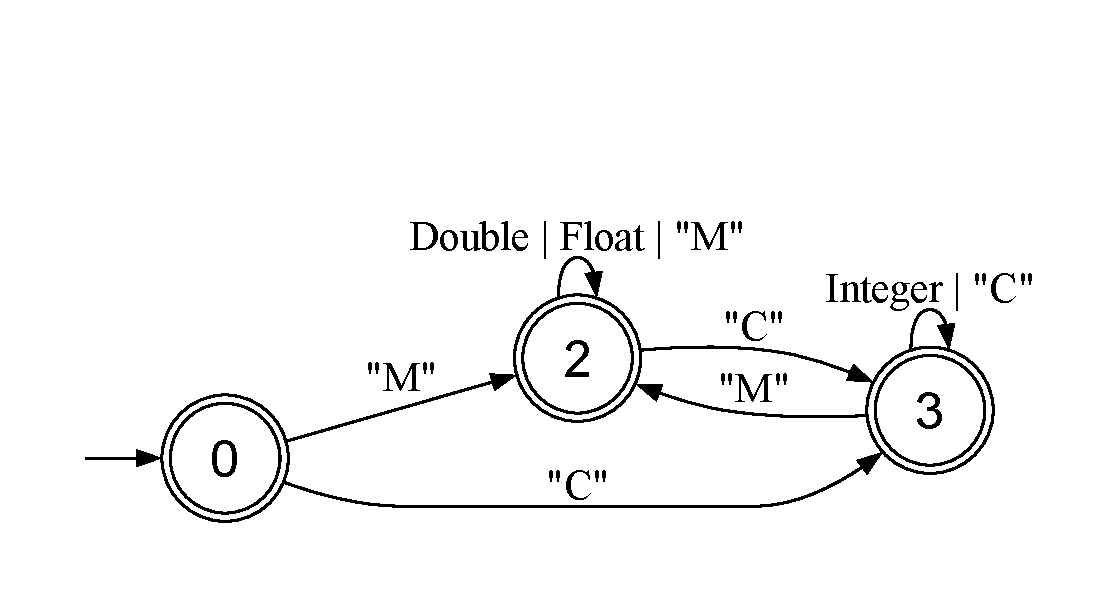
\includegraphics[height=0.5\textheight,trim = {1.8cm 1.0cm 0 3.5cm}, clip]{example2.pdf}
\end{frame}
